\section{Equations of motion}

In this section we derive the equation of motion for a driven, damped Josephson oscillator with parametric modulation of its inductance.

\subsection{Josephson oscillator}

Consider a parallel resistor $R$, capacitor $C$, and Josephson junction of critical current $I_c$, driven by an external current source $I_s(t) = I_s \cos(\omega_s t + \theta)$.
The equation of motion for this circuit is
\begin{equation}
\ddot{\phi} + \frac{1}{RC}\dot{\phi} + \frac{1}{L_{J_0}C}\sin \phi = \frac{2\pi}{C \Phi_0} I_s \cos(\omega_s t + \theta)
\end{equation}
where $L_{J_0} \equiv \Phi_0 / 2\pi I_c$ is the un-biased inductance of the junction.
Defining $\omega_0 \equiv 1 / \sqrt{L_{J_0}C}$, $2 \Gamma \equiv 1/RC$, and $J \equiv  2\pi I_s / C \Phi_0$, we can re-write the equation of motion as
\begin{equation}
\ddot{\phi} + 2\Gamma \dot{\phi} + \omega_0^2 \sin \phi = J \cos(\omega_s t + \theta) .
\end{equation}

\subsection{Parametric pumping}

Suppose the junction were instead a DC SQUID. We could then modulate the inductance by driving flux through the SQUID loop. The inductance of the SQUID is then \begin{equation}
L(t) = L_{\textrm{dc}} + \Phi_p \frac{dL}{d\Phi}\cos(\omega_p t) \end{equation}
where $L_{\textrm{dc}}$ is the inductance of the SQUID under a constant flux bias, and $\Phi_p$ is the amplitude of the flux drive signal. This leads to a time dependent oscillation frequency \begin{eqnarray}
\omega_0(t) &=& (L_{\textrm{dc}}C)^{-1/2} \left(1 + \cos(\omega_p t) \frac{dL/L_{\textrm{dc}}} {d\Phi/\Phi_p} \right)^{-1/2} \\
&\approx& \omega_{0,\textrm{dc}} \left( 1 -\cos(\omega_p t) \frac{1}{2}\frac{dL/L_{\textrm{dc}}}{d\Phi/\Phi_p} \right) \\
&\equiv& \omega_{0,\textrm{dc}}\left( 1 - A\cos(\omega_p t) \right) \end{eqnarray}

Now the equation of motion is \begin{equation}
\ddot{\phi} + 2\Gamma \dot{\phi} + \omega_{0,\textrm{dc}}^2(1 - A \cos(\omega_p t))\sin(\phi) = J\cos(\omega_s t + \theta) \end{equation}
Taking only the linear term of the $\sin$ we get \begin{equation}
\ddot{\phi} + 2\Gamma \dot{\phi} + \omega_{0,\textrm{dc}}^2(1 - A \cos(\omega_p t))\phi = J\cos(\omega_s t + \theta) \label{eq:motion} \end{equation}
which is a driven, damped harmonic oscillator with time dependent frequency.

\section{Solution of equations of motion}

Equation (\ref{eq:motion}) is best studied in the frequency domain.
Making the transformation to frequency is easy using the following facts \begin{eqnarray}
\cos(\Omega t + \theta) &\rightarrow& \frac{1}{2}(2\pi)\left(e^{i \theta}\delta(\omega - \Omega) + e^{-i \theta} \delta(\omega + \Omega) \right) \nonumber \\
\phi(t)\cos(\Omega t) &\rightarrow& \frac{1}{2}\left( \tilde{\phi}(\omega-\Omega) + \tilde{\phi}(\omega+\Omega) \right) \nonumber \\
\dot{\phi}(t) &\rightarrow& i\omega \tilde{\phi}(\omega) \nonumber \end{eqnarray}
Using these equations and defining $L(\omega) \equiv (\omega_0^2 - \omega^2 +i2\omega\Gamma)$, we get
\begin{equation*}
  \underbrace{L(\omega) \tilde{\phi}(\omega)}_{\text{linear response}}
  - \underbrace{\frac{1}{2} A \omega_0^2 \left[ \tilde{\phi}(\omega - \omega_p) + \tilde{\phi}(\omega + \omega_p) \right]}_{\text{modulated response}}
  = \underbrace{\frac{1}{2}J(2\pi)\left[e^{i \theta}\delta(\omega-\omega_s) + e^{-i\theta}\delta(\omega+\omega_s) \right]}_{\text{source}} \, .
\end{equation*}
It's useful to use a simplified notation where $\ket{\omega}$ indicates a delta function peak at frequency $\omega$ and $T_{\omega}$ indicates a shift in frequency by an amount $\omega$.
In this new notation, we have
\begin{equation}
  \left(
      \underbrace{L(\omega)}_{\text{linear response}}
    - \underbrace{
        \frac{1}{2} A \omega_0^2
        \left[
          T_{\omega_p} + T_{-\omega_p}
        \right]
      }_{\text{modulated response}}
  \right) \ket{\phi}
  = \underbrace{\frac{1}{2} J (2\pi) \left[e^{i \theta} \ket{\omega_s} + e^{-i \theta} \ket{-\omega_s} \right]}_{\text{source}}
  \, . \label{eq:eqOfMotionFrequency}
\end{equation}
We want to solve for $\ket{\phi}$.
If the parametric modulation were absent ($A=0$), then we would get the standard driven harmonic oscillator equation and $\phi$ would be a single tone at $\omega_s$.
To seed this, let us try the solution
\begin{align*}
  \phi(t) =& a \cos(\omega_s t + \varphi) \\
  \rightarrow \ket{\phi} =& \frac{1}{2} \left( \alpha \ket{\omega_s} + \alpha^* \ket{-\omega_s} \right) \, .
\end{align*}
where $\alpha \equiv a e^{i \varphi}$.
Plugging into Eq. (\ref{eq:eqOfMotionFrequency}) and equating coefficients of the like frequency components on either side gives
\begin{displaymath}
  L(\omega_s) \alpha = J (2 \pi) e^{i \theta}
  \qquad \text{and} \qquad
  L(-\omega_s) \alpha^* = J (2 \pi) e^{-i \theta} \, ,
\end{displaymath}
which solve for $\alpha$ in terms of the drive amplitude and phase, and the linear response function $L$.
Note that the equations for $\alpha$ and $\alpha^*$ are degenerate because $L(-\omega) = L(\omega)^*$.

\begin{figure}
\begin{centering}
\includegraphics[width=\textwidth]{response_balance.pdf}
\par\end{centering}
\caption{The three terms in Eq. (\ref{eq:eqOfMotionFrequency}).
a) The source term is a pure tone at $\omega_s$.
Assuming $\ket{\phi}$ is also a pure tone at $\omega_s$ (shown in blue), the linear response term produces scaled peaks at $\pm \omega_s$.
The modulated response produces a copy of $\ket{\phi}$ shifted by $\omega_p$; we show only the right-shifted part, and we ignore the high frequency peaks at $\pm (\omega_s + \omega_p)$.
In this case, the linear and modulated response terms do not sum up to match the source because there's an ``extra'' peak to the left of $\omega_p/2$.
b) Here $\ket{\phi}$ includes another tone at $\omega_i$ with amplitude $\beta$ (red).
Now we can choose $\alpha$ and $\beta$ such that the linear and modulated responses sum to match the source.}
\label{Fig:responseBalance}
\end{figure}

The parametric drive produces frequency-shifted copies of $\ket{\phi}$ so a single tone solution at $\omega_s$ does not solve Eq. (\ref{eq:eqOfMotionFrequency}).
To understand how to fix this, we construct a diagram representing the right and left hand sides of Eq. (\ref{eq:eqOfMotionFrequency}), as shown in Figure \ref{Fig:responseBalance}.
Figure \ref{Fig:responseBalance}a shows the frequency space representation of the source and response terms in Eq. \ref{eq:eqOfMotionFrequency}) assuming that $\ket{\phi}$ a single tone at $\omega_s$ with amplitude $\alpha$, and also assuming that $\omega_p \approx 2 \omega_s$.
Adding the linear and modulated responses gives a tone with amplitude $\alpha^*$ at frequency $\omega_i \equiv \omega_p - \omega_s$ that has no counterpart in the source.
The only solution in this case is $\alpha=0$, which is trivial.

The diagram suggests solution: suppose the response has another tone at frequency $\omega_i$ with amplitude $\beta$ as shown by the red peaks in Figure \ref{Fig:responseBalance}b.
Now the frequency shifted copies can add both to match the source at $\omega_s$ and, if the amplitudes are chosen correctly, to cancel at $\omega_i$.
The response peak at $\omega_s$ is called the ``signal'' and the peak at $\omega_i$ is called the ``idler''.

Let us now do the math carefully.
We take the guess
\begin{align*}
  \phi(t) =& a \cos(\omega_s t + \varphi_a) + b \cos(\omega_i t + \varphi_b) \\
  \rightarrow
  \ket{\phi} =& \frac{1}{2}(2\pi)
  \left(
      \alpha \ket{\omega_s} + \alpha^* \ket{-\omega_s}
    + \beta  \ket{\omega_i} + \beta^*  \ket{-\omega_i}
    \right)
\end{align*}
Plugging into Eq. (\ref{eq:eqOfMotionFrequency}) and keeping only the positive frequency terms for simplicity\footnote{No generality is lost here.}, and \emph{dropping high frequency terms} we find
\begin{equation*}
    L(\omega_s) \alpha \ket{\omega_s}
  + L(\omega_i) \beta  \ket{\omega_i}
  - \frac{A \omega_0^2}{2} \alpha^* \ket{\omega_i}
  - \frac{A \omega_0^2}{2} \beta^*  \ket{\omega_s}
  = J e^{i \theta} \ket{\omega_s} \, .
\end{equation*}
Equating coefficients of like frequency terms yields two equations:
\begin{align*}
  L(\omega_s)\alpha - \frac{A \omega_0^2}{2} \beta^* =& J e^{i \theta} \\
  L(\omega_i)\beta - \frac{A \omega_0^2}{2} \alpha^* =& 0 .
\end{align*}
Solving the two simultaneous equations gives
\begin{equation}
  \alpha = \frac{L(\omega_i)^* J e^{i\theta}}{L(\omega_s)L(\omega_i)^* - (A \omega_0^2/2)^2}
  \, . \label{eq:alphabeta}
\end{equation}
In Figure \ref{Fig:response} we plot the magnitude of $\alpha$ for a few values of the pump amplitude.

\begin{figure}
\begin{centering}
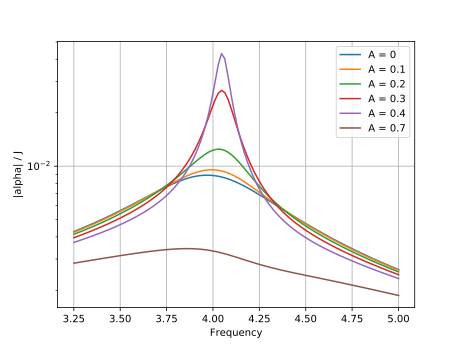
\includegraphics[width=\textwidth]{response.pdf}
\par\end{centering}
\caption{Magnitude of $\alpha/J$ as a function of linear (not angular) drive frequency $\omega_s$ for a few values of the pump amplitude $A$.
Here we have $\omega_0/2\pi = 4$, $\omega_p/2\pi = 8.1$, $Q = \omega_0/2\Gamma = 5.6$.
}
\label{Fig:response}
\end{figure}
